\section{Tugas 2}
\subsection{Teori}
\begin{enumerate}
\item Integer, Boolean, Char, Float, String
\begin{figure}
\item input()
\centering
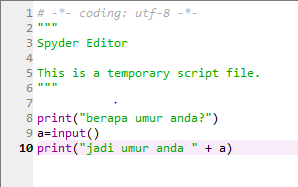
\includegraphics[width=6cm,height=6cm]{figures/c1.png}
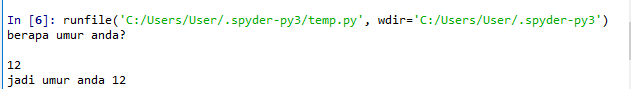
\includegraphics[width=6cm,height=6cm]{figures/c2.png}
\caption {input dan outputnya}
\end{figure}
\begin{figure}
\item asd
\centering
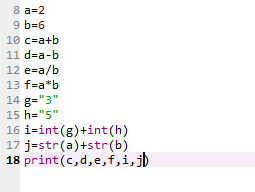
\includegraphics[width=6cm,height=6cm]{figures/c3.png}
\caption{operasi aritmatika}
\end{figure}
\begin{figure}
\item loop digunakan untuk mengulang sampai memenuhi sebuah condition, contoh :
\centering
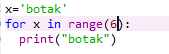
\includegraphics[width=6cm,height=6cm]{figures/c4.png}
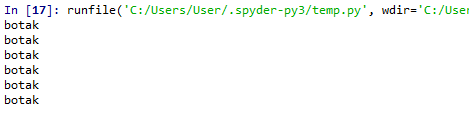
\includegraphics[width=6cm,height=6cm]{figures/c5.png}
\caption {contoh loop/pengulangan}
\end{figure}
\begin{figure}
\item memilih kondisi menggukan syntax if else, cara memakainya yaitu jika sebuah kondisi tidak terpenuhi makan akan meng-execute kondisi lain. contoh:
\centering
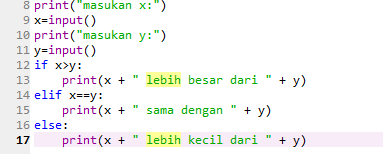
\includegraphics[width=6cm,height=6cm]{figures/c6.png}
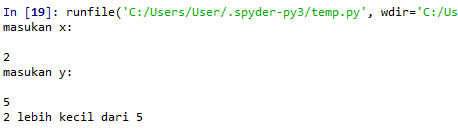
\includegraphics[width=6cm,height=6cm]{figures/c7.png}
\caption{contoh syntax kondisi}
\end{figure}
\begin{figure}
\item asd
\end{figure}
\begin{figure}
\item try berfungsi untuk menguji error, exept berfungsi untuk menangani error. cara memakainya :
\centering
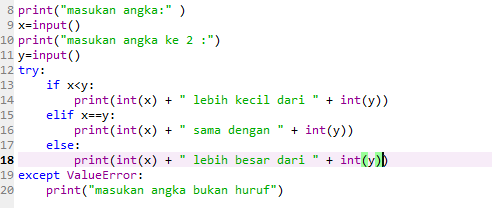
\includegraphics[width=6cm,height=6cm]{figures/c8.png}
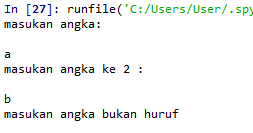
\includegraphics[width=6cm,height=6cm]{figures/c9.png}
\caption{contoh try except}
\end{figure}
\end{enumerate}
\begin{figure}
\subsection{Keterampilan Pemrograman}
\end{figure}
\begin{enumerate}
\begin{figure}
\item a
\end{figure}
\begin{figure}
\item
\center
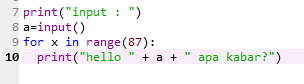
\includegraphics[width=6cm,height=6cm]{figures/c10.png}
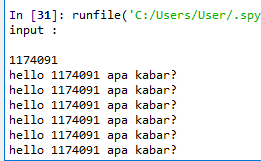
\includegraphics[width=6cm,height=6cm]{figures/c11.png}
\end{figure}
\begin{figure}
\item
\center
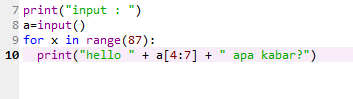
\includegraphics[width=6cm,height=6cm]{figures/c12.png}
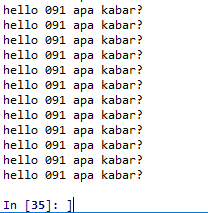
\includegraphics[width=6cm,height=6cm]{figures/c13.png}
\end{figure}
\begin{figure}
\item
\center
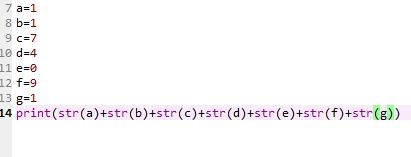
\includegraphics[width=6cm,height=6cm]{figures/c15.png}
\end{figure}
\begin{figure}
\item
\center
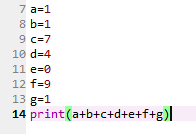
\includegraphics[width=6cm,height=6cm]{figures/c16.png}
\end{figure}
\begin{figure}
\item
\center
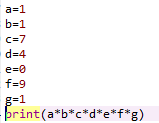
\includegraphics[width=6cm,height=6cm]{figures/c17.png}
\end{figure}
\begin{figure}
\item
\center
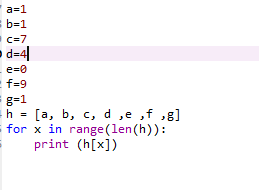
\includegraphics[width=6cm,height=6cm]{figures/c18.png}
\end{figure}
\begin{figure}
\item
\center
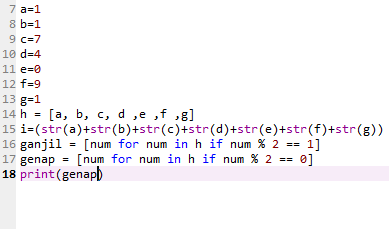
\includegraphics[width=6cm,height=6cm]{figures/c19.png}
\end{figure}
\begin{figure}
\item
\center
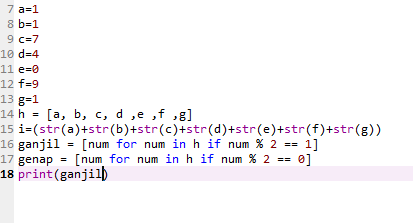
\includegraphics[width=6cm,height=6cm]{figures/c20.png}
\end{figure}
\begin{figure}
\item
\center
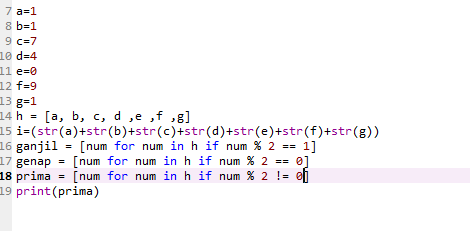
\includegraphics[width=6cm,height=6cm]{figures/c21.png}
\end{figure}
\end{enumerate}